\documentclass[conference]{IEEEtran}
\usepackage[utf8]{inputenc}
\usepackage[T1]{fontenc}
\usepackage[brazil]{babel}
\usepackage{graphicx}
\usepackage{booktabs}
\usepackage{amsmath}
\usepackage{url}
\usepackage{xcolor}
% Marcador para dados que a equipe precisa fornecer (nomes, links).
\newcommand{\todo}[1]{\textbf{\textcolor{red}{[#1]}}}
\graphicspath{{figuras/}}

\begin{document}

\title{EcoAssist: Assistente de Descarte de Res\'iduos Integrando Vis\~ao Computacional, Processamento de Linguagem Natural e Decis\~ao Baseada em Regras}

\author{\IEEEauthorblockN{\todo{Nome completo 1}, \todo{Nome completo 2}, \todo{Nome completo 3}}
\IEEEauthorblockA{Curso de \todo{curso}, AFYA | UNIMA Macei\'o, Brasil\\
Disciplina de Intelig\^encia Artificial -- Prof. Icaro Ferreira}}

\maketitle

\begin{abstract}
O descarte incorreto de res\'iduos reduz a efici\^encia da coleta seletiva, e a d\'uvida sobre \emph{como} descartar cada item \'e uma das causas. Este trabalho apresenta o EcoAssist, aplica\c{c}\~ao que recebe a foto de um res\'iduo e uma pergunta em portugu\^es e responde com a orienta\c{c}\~ao de descarte e a fonte utilizada. Em um \'unico fluxo, o sistema integra um classificador visual MobileNetV2 ajustado por \emph{transfer learning} no conjunto TrashNet, um m\'odulo de PLN com reconhecimento de inten\c{c}\~ao (TF-IDF e Regress\~ao Log\'istica), extra\c{c}\~ao do material citado e busca sem\^antica, e um agente baseado em regras que combina as confian\c{c}as da imagem e do texto. No teste do TrashNet, a MobileNetV2 obteve acur\'acia de 0{,}882 e F1 macro de 0{,}865, contra 0{,}611 e 0{,}582 de uma linha de base HOG+SVM. Em 48 pares (imagem de teste e pergunta escrita livremente), a avalia\c{c}\~ao inicial obteve 54{,}2\% de acerto de ponta a ponta, limitado pelo PLN treinado com frases sint\'eticas. Ap\'os ajustes guiados por esses mesmos pares, o acerto chegou a 66{,}7\%, valor tratado como resultado de desenvolvimento. Discutem-se casos de baixa confian\c{c}a, perguntas compostas e a necessidade de avalia\c{c}\~ao com fotos reais.
\end{abstract}

\begin{IEEEkeywords}
vis\~ao computacional, processamento de linguagem natural, \emph{transfer learning}, res\'iduos, sistemas baseados em regras
\end{IEEEkeywords}

\section{Introdu\c{c}\~ao}
A coleta seletiva depende da separa\c{c}\~ao correta dos res\'iduos pelo cidad\~ao. No Brasil, a Resolu\c{c}\~ao CONAMA n\textordmasculine{} 275/2001 padroniza as cores dos coletores~\cite{conama275}, mas d\'uvidas pr\'aticas persistem: qual \'e o material, se ele \'e recicl\'avel, se precisa ser lavado. Um assistente que identifique o material por foto e responda a perguntas em linguagem natural pode reduzir essa barreira.

O objetivo deste trabalho \'e projetar, implementar e avaliar um sistema que integre Aprendizado de M\'aquina, Vis\~ao Computacional e PLN em um mesmo fluxo funcional, mediado por um componente de decis\~ao. As contribui\c{c}\~oes s\~ao: (i) uma arquitetura em que imagem e pergunta s\~ao combinadas por um agente de regras sens\'ivel \`a confian\c{c}a; (ii) uma avalia\c{c}\~ao que compara o modelo de imagens com uma linha de base cl\'assica e mede o sistema de ponta a ponta, separando resultado inicial e de desenvolvimento; e (iii) um reposit\'orio reproduz\'ivel: \todo{URL do GitHub}.

\section{Fundamenta\c{c}\~ao e Trabalhos Relacionados}
\textbf{\emph{Transfer learning.}} Redes convolucionais pr\'e-treinadas no ImageNet podem ser adaptadas a tarefas com poucos dados substituindo e retreinando suas camadas finais. A MobileNetV2~\cite{sandler2018} usa blocos residuais invertidos com convolu\c{c}\~oes separ\'aveis em profundidade, o que a torna adequada \`a execu\c{c}\~ao em CPU.

\textbf{Classifica\c{c}\~ao de res\'iduos.} O TrashNet~\cite{yang2016} re\'une cerca de 2500 imagens de seis classes (papel\~ao, vidro, metal, papel, pl\'astico e rejeito) sobre fundo uniforme; no trabalho original, um SVM sobre descritores de imagem superou a rede convolucional treinada do zero. Aral \emph{et al.}~\cite{aral2018} compararam arquiteturas pr\'e-treinadas (DenseNet, Inception-ResNet, MobileNet e Xception) no TrashNet com aumento de dados, e Bircanoglu \emph{et al.}~\cite{bircanoglu2018} propuseram a RecycleNet, obtendo os melhores resultados com DenseNet121 ajustada a partir do ImageNet. Esses trabalhos tratam apenas da classifica\c{c}\~ao visual; o EcoAssist acrescenta a interpreta\c{c}\~ao da pergunta e a decis\~ao sobre a resposta.

\textbf{Linha de base cl\'assica.} Histogramas de gradientes orientados (HOG)~\cite{dalal2005} combinados com SVM~\cite{cortes1995} s\~ao uma refer\^encia cl\'assica de extra\c{c}\~ao de caracter\'isticas.

\textbf{PLN.} A representa\c{c}\~ao TF-IDF com um classificador linear \'e uma linha de base robusta para reconhecimento de inten\c{c}\~oes. Para busca sem\^antica, o Sentence-BERT~\cite{reimers2019} gera vetores de senten\c{c}as comparados pela similaridade do cosseno.

\textbf{Decis\~ao.} Agentes baseados em regras e em utilidade combinam evid\^encias incertas de forma expl\'icita e audit\'avel~\cite{russell2020}, o que permite justificar cada resposta ao usu\'ario.

\section{Metodologia}
\subsection{Arquitetura}
A Fig.~\ref{fig:arq} mostra o fluxo. A imagem passa pelo classificador visual, que devolve as tr\^es classes mais prov\'aveis com suas probabilidades. A pergunta passa pelo PLN, que devolve a inten\c{c}\~ao e sua confian\c{c}a, o material eventualmente citado e os trechos recuperados da base de conhecimento. O agente de decis\~ao combina essas sa\'idas e gera a resposta exibida na interface Streamlit, junto com a regra aplicada.

\begin{figure}[t]
\centering
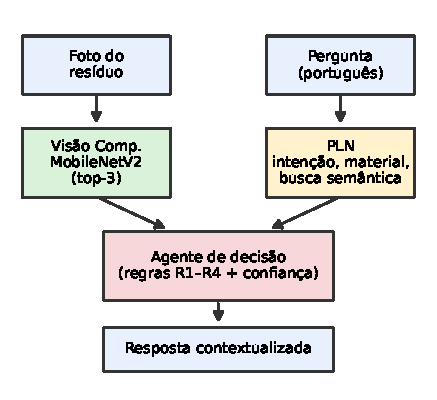
\includegraphics[width=0.78\columnwidth]{arquitetura.pdf}
\caption{Arquitetura do EcoAssist.}
\label{fig:arq}
\end{figure}

\subsection{Dados}
\emph{Imagens:} TrashNet~\cite{yang2016}, 2527 imagens, divididas de forma estratificada em 70/15/15\% (1768 de treino, 379 de valida\c{c}\~ao e 380 de teste), semente 42. Aumento de dados (espelhamento, rota\c{c}\~ao de at\'e 15$^\circ$ e brilho) foi aplicado apenas ao treino.

\emph{Texto:} seis inten\c{c}\~oes (como descartar, identificar material, recicl\'avel, cor da lixeira, cuidados e curiosidade). A vers\~ao inicial usou 340 frases sint\'eticas geradas por modelos de frases; a vers\~ao ajustada acrescentou 69 frases escritas \`a m\~ao. Para avalia\c{c}\~ao, foram escritas 48 perguntas livres (8 por inten\c{c}\~ao), com apoio de ferramenta de IA generativa, fora dos modelos de frase.

\emph{Base de conhecimento:} orienta\c{c}\~oes de descarte por classe (lixeira, reciclabilidade, cuidados) e dez trechos, com cores de coletores segundo a Resolu\c{c}\~ao CONAMA 275/2001~\cite{conama275}.

\subsection{Modelos}
A MobileNetV2 teve a camada final substitu\'ida por uma camada linear de seis sa\'idas. Treinou-se primeiro apenas essa camada (Adam, taxa $10^{-3}$) e, a partir da quarta \'epoca, tamb\'em os quatro \'ultimos blocos (taxa $10^{-4}$), com lotes de 32 e 6 \'epocas, em PyTorch~\cite{paszke2019}. A linha de base usa HOG sobre imagens $128\times128$ em tons de cinza e SVM com n\'ucleo RBF ($C=10$), em scikit-learn~\cite{pedregosa2011}. A inten\c{c}\~ao usa TF-IDF de uni e bigramas e Regress\~ao Log\'istica. A busca usa o modelo \texttt{paraphrase-multilingual-MiniLM-L12-v2}~\cite{reimers2019}, com contingência TF-IDF quando o modelo n\~ao est\'a dispon\'ivel.

\subsection{Agente de decis\~ao}
As regras s\~ao: \textbf{R1} confian\c{c}a visual $<0{,}60$ e nenhum material no texto: pede nova foto; \textbf{R2} confian\c{c}a visual baixa e material citado no texto: usa o texto; \textbf{R3} texto contradiz imagem confiante: a imagem prevalece, com aviso; \textbf{R4} caso padr\~ao: usa a imagem. A vers\~ao ajustada acrescenta \textbf{R5}: confian\c{c}a da inten\c{c}\~ao $<0{,}40$ gera uma resposta-resumo (material, reciclabilidade, lixeira e descarte) em vez de assumir uma inten\c{c}\~ao. Os limiares foram fixados a priori.

\subsection{Protocolo de avalia\c{c}\~ao e m\'etricas}
Para imagens: acur\'acia, F1 macro e matriz de confus\~ao no teste. Para inten\c{c}\~oes: acur\'acia e F1 macro nas 48 perguntas livres. Para o sistema: 48 pares formados por imagens do teste do TrashNet (8 por classe) e perguntas livres; um par \'e correto quando a classe final coincide com a real e a inten\c{c}\~ao prevista com a esperada. A avalia\c{c}\~ao \emph{inicial} foi feita antes de qualquer ajuste no PLN. Em seguida, os erros dessas mesmas perguntas guiaram os ajustes (frases extras, regulariza\c{c}\~ao $C=10$, R5, busca restrita \`a classe prevista e embeddings); por isso, os n\'umeros da vers\~ao ajustada s\~ao \emph{resultado de desenvolvimento}, otimistas. A avalia\c{c}\~ao final prevista usa pares novos com fotos de celular e respostas esperadas definidas antes do uso do aplicativo, n\~ao realizada nesta vers\~ao. Tudo foi executado em CPU.

\section{Resultados e Discuss\~ao}
\subsection{Vis\~ao computacional}
A Tabela~\ref{tab:img} mostra que a transfer\^encia de aprendizado elevou a acur\'acia em 27 pontos percentuais sobre a linha de base. Na matriz de confus\~ao (Fig.~\ref{fig:cm}), os principais erros s\~ao papel\~ao classificado como papel (7 de 60), vidro como metal (6 de 76) e pl\'astico como vidro ou metal (9 de 73). A classe \emph{rejeito}, com menos exemplos, acertou 12 de 20 imagens.

\begin{table}[t]
\centering
\caption{Desempenho no conjunto de teste de imagens ($n=380$).}
\label{tab:img}
\begin{tabular}{lcc}
\toprule
Modelo & Acur\'acia & F1 macro\\
\midrule
HOG + SVM & 0,611 & 0,582\\
MobileNetV2 & 0,882 & 0,865\\
\bottomrule
\end{tabular}
\end{table}

\begin{figure}[t]
\centering
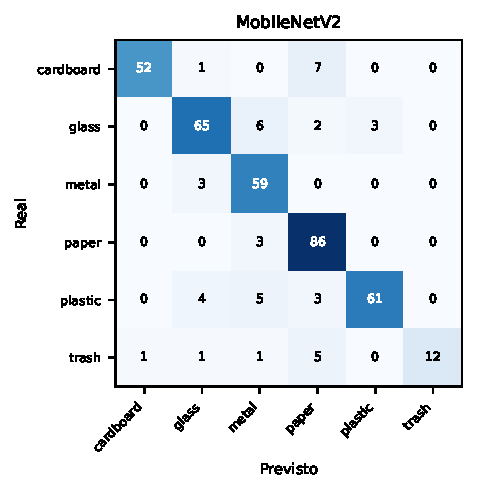
\includegraphics[width=0.82\columnwidth]{matriz_confusao_mobilenetv2.pdf}
\caption{Matriz de confus\~ao da MobileNetV2 no teste do TrashNet.}
\label{fig:cm}
\end{figure}

\subsection{PLN e sistema integrado}
A Tabela~\ref{tab:sis} resume os resultados. Na vers\~ao inicial, a inten\c{c}\~ao alcan\c{c}ou F1 igual a 1{,}0 no teste sint\'etico, mas 0{,}65 de acur\'acia nas perguntas livres: o vocabul\'ario de treino tinha apenas 297 termos (uni e bigramas), dominados pelos objetos dos modelos de frase, e palavras como ``perigoso'', ``balde'' e ``benef\'icio'' estavam ausentes. Todos os 17 erros tiveram confian\c{c}a abaixo de 0{,}50. No sistema integrado, a classe visual estava correta em 87{,}5\% dos pares, a classe final decidida pelo agente em 81{,}3\% e o acerto conjunto foi 54{,}2\%, de modo que o PLN era o limitante.

\begin{table}[t]
\centering
\caption{Inten\c{c}\~ao (48 perguntas livres) e sistema (48 pares).}
\label{tab:sis}
\begin{tabular}{lcc}
\toprule
M\'etrica & Inicial & Desenvolv.$^{*}$\\
\midrule
Acur\'acia de inten\c{c}\~ao & 0,65 & 0,90\\
Classe final correta & 81,3\% & 81,3\%\\
Acerto de ponta a ponta & 54,2\% & 66,7\%\\
\bottomrule
\multicolumn{3}{l}{\footnotesize $^{*}$Ajustes guiados pelos mesmos 48 pares; valores otimistas.}
\end{tabular}
\end{table}

Ap\'os os ajustes, a inten\c{c}\~ao chegou a 0{,}90 e o acerto de ponta a ponta a 66{,}7\%. Como as mesmas perguntas orientaram os ajustes, inclusive a escolha de $C$, esse ganho n\~ao representa desempenho em dados novos; a classe final n\~ao mudou porque o modelo visual n\~ao foi alterado.

\textbf{Baixa confian\c{c}a.} A regra R1 foi acionada em 5 dos 48 pares. Em 3 deles a classe mais prov\'avel estava errada (papel\~ao $\rightarrow$ vidro com 0{,}29; pl\'astico $\rightarrow$ vidro com 0{,}29; rejeito $\rightarrow$ papel com 0{,}33), e o agente pediu nova foto em vez de responder errado; nos outros 2 a classe estava certa com confian\c{c}a baixa (0{,}52 e 0{,}34). Os erros visuais tiveram confian\c{c}a m\'edia de 0{,}51, contra 0{,}84 nos acertos, mas tr\^es erros ultrapassaram o limiar (0{,}63 a 0{,}85) e geraram respostas incorretas. A regra R5 foi acionada em 12 pares da vers\~ao ajustada; neles, a inten\c{c}\~ao mais prov\'avel estava certa em apenas 33\% dos casos, o que justifica responder com um resumo.

\textbf{Conflitos texto--imagem.} Na avalia\c{c}\~ao inicial, os 7 casos de R3 decorreram de men\c{c}\~oes que n\~ao afirmavam o material: termos gen\'ericos como ``lixo'' (associado a rejeito) e ``garrafa'' (associado a pl\'astico), ou perguntas com alternativas, como ``\'e pl\'astico ou vidro?''. A imagem prevaleceu corretamente em 6 deles.

\textbf{Pergunta composta.} Em teste manual no aplicativo, a pergunta ``em qual cor de lixeira da coleta seletiva isso entra, e precisa lavar antes?'', com foto de metal (confian\c{c}a 0{,}87), recebeu apenas a cor da lixeira e a fonte sobre o c\'odigo de cores; a parte sobre lavagem foi ignorada, pois o PLN atribui uma \'unica inten\c{c}\~ao por pergunta.

\subsection{Limita\c{c}\~oes}
O TrashNet tem fundo uniforme, o que tende a superestimar o desempenho em fotos reais, e os pares de avalia\c{c}\~ao usam imagens desse mesmo conjunto. As inten\c{c}\~oes de treino s\~ao majoritariamente sint\'eticas e as perguntas livres foram escritas com apoio de IA. A base de conhecimento \'e pequena e as regras de coleta variam por munic\'ipio. O sistema n\~ao trata m\'ultiplos objetos na mesma imagem nem perguntas com v\'arias partes, e a extra\c{c}\~ao do material por palavras-chave gera falsos conflitos. A busca sem\^antica n\~ao teve avalia\c{c}\~ao quantitativa pr\'opria.

\section{Conclus\~ao e Trabalhos Futuros}
O EcoAssist integra classifica\c{c}\~ao visual, PLN e decis\~ao por regras em um fluxo \'unico e demonstr\'avel. A MobileNetV2 alcan\c{c}ou 88{,}2\% de acur\'acia no TrashNet, e o agente evitou respostas erradas em parte dos casos de baixa confian\c{c}a. O PLN foi o principal limitante: o acerto de ponta a ponta foi de 54{,}2\% na avalia\c{c}\~ao inicial e de 66{,}7\% ap\'os ajustes, este \'ultimo um resultado de desenvolvimento. Como trabalhos futuros: avaliar com fotos de celular e perguntas in\'editas, j\'a preparado no reposit\'orio; coletar perguntas reais para treinar a inten\c{c}\~ao; tratar perguntas compostas com classifica\c{c}\~ao multirr\'otulo; usar detec\c{c}\~ao de objetos para m\'ultiplos itens; e calibrar os limiares de confian\c{c}a em um conjunto de valida\c{c}\~ao.

\begin{thebibliography}{00}
\bibitem{yang2016} M. Yang and G. Thung, ``Classification of trash for recyclability status,'' Stanford CS229 Project, 2016. [Online]. Available: \url{https://github.com/garythung/trashnet}
\bibitem{conama275} Conselho Nacional do Meio Ambiente (CONAMA), ``Resolu\c{c}\~ao n\textordmasculine{} 275, de 25 de abril de 2001: estabelece o c\'odigo de cores para os diferentes tipos de res\'iduos,'' \emph{Di\'ario Oficial da Uni\~ao}, 19 jun. 2001.
\bibitem{sandler2018} M. Sandler, A. Howard, M. Zhu, A. Zhmoginov, and L.-C. Chen, ``MobileNetV2: Inverted residuals and linear bottlenecks,'' in \emph{Proc. IEEE/CVF Conf. Computer Vision and Pattern Recognition (CVPR)}, 2018, pp. 4510--4520, doi: 10.1109/CVPR.2018.00474.
\bibitem{aral2018} R. A. Aral, S. R. Keskin, M. Kaya, and M. Hac\i{}\"omero\u{g}lu, ``Classification of TrashNet dataset based on deep learning models,'' in \emph{Proc. IEEE Int. Conf. Big Data}, 2018, pp. 2058--2062.
\bibitem{bircanoglu2018} C. Bircano\u{g}lu, M. Atay, F. Be\c{s}er, \"O. Gen\c{c}, and M. A. K\i{}zrak, ``RecycleNet: Intelligent waste sorting using deep neural networks,'' in \emph{Proc. IEEE Int. Conf. Innovations in Intelligent Systems and Applications (INISTA)}, 2018.
\bibitem{dalal2005} N. Dalal and B. Triggs, ``Histograms of oriented gradients for human detection,'' in \emph{Proc. IEEE CVPR}, 2005, pp. 886--893.
\bibitem{cortes1995} C. Cortes and V. Vapnik, ``Support-vector networks,'' \emph{Machine Learning}, vol. 20, no. 3, pp. 273--297, 1995.
\bibitem{reimers2019} N. Reimers and I. Gurevych, ``Sentence-BERT: Sentence embeddings using Siamese BERT-networks,'' in \emph{Proc. EMNLP-IJCNLP}, 2019, pp. 3982--3992, doi: 10.18653/v1/D19-1410.
\bibitem{paszke2019} A. Paszke \emph{et al.}, ``PyTorch: An imperative style, high-performance deep learning library,'' in \emph{Advances in Neural Information Processing Systems 32}, 2019, pp. 8024--8035.
\bibitem{pedregosa2011} F. Pedregosa \emph{et al.}, ``Scikit-learn: Machine learning in Python,'' \emph{J. Machine Learning Research}, vol. 12, pp. 2825--2830, 2011.
\bibitem{russell2020} S. Russell and P. Norvig, \emph{Artificial Intelligence: A Modern Approach}, 4th ed. Hoboken, NJ, USA: Pearson, 2020.
\end{thebibliography}

\end{document}
